\chapter{Mezclador de Transmisión}
\label{section:mezcla}

En este Capítulo se describe el último bloque del sistema, correspondiente al mezclador de transmisión. Este bloque se compone de tres procesos: la generación de señales sinusoidales mediante un sintetizador de señal (DDS), la multiplicación de los datos I/Q por estas señales sinusoidales y la suma final de las componentes I/Q de transmisión. En la Figura \ref{fig:mezclador} se visualiza la estructura de los bloques IP que se han incluido en este tercer proyecto de Vivado.

\begin{figure}[h]
    \centering
    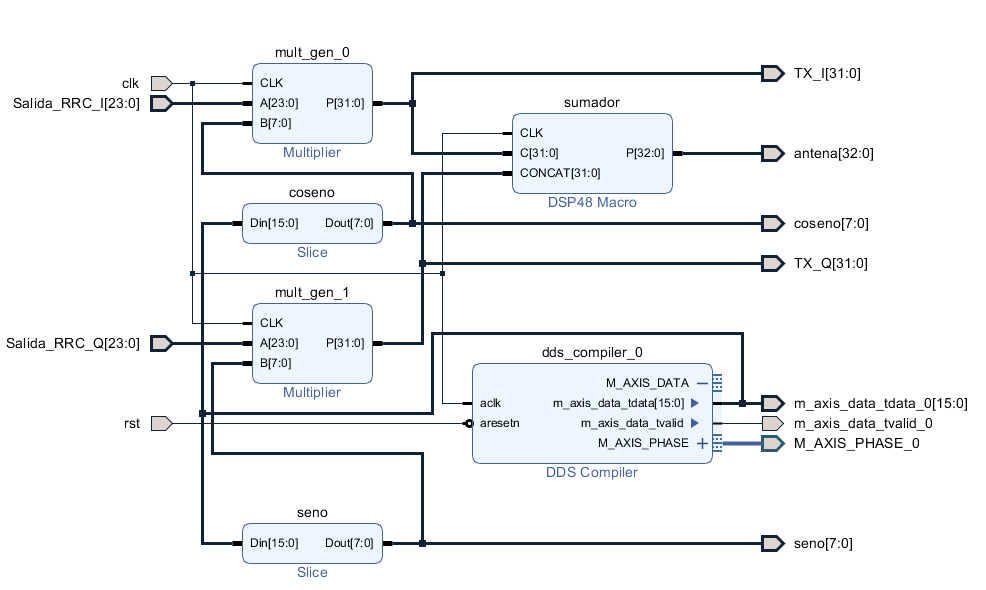
\includegraphics[width=1.05\textwidth, height=10cm]{img/diseno/mezclador.PNG}
    \caption{Diseño del bloque mezclador de transmisión}
    \label{fig:mezclador}
\end{figure}

\pagebreak

\section{Generación de las sinusoides}

Se deben generar dos señales sinusoidales, en particular una función coseno y otra -seno, a partir de un bloque DDS (\textit{Direct Digital Synthesis}). Este bloque es capaz de generar señales analógicas de forma directa mediante un oscilador controlado numéricamente (NCO) y para ello, es preciso configurar internamente la frecuencia de salida deseada de las señales. En el caso de este proyecto será de 100MHz y el reloj del sistema tendrá una frecuencia de 576MHz (3x192MHz), por lo que se obtendrán 5/6 muestras por ciclo.

\vspace{3mm}

La salida del bloque DDS (\textit{m\_axis\_data\_tdata}) esta constituida por 16 bits, de los cuales 8 corresponderán a la señal de seno y los otros 8, a la de coseno como se puede apreciar en la Figura \ref{fig:dds}. Es por ello que se requiere dividir la salida y definir los bits que se dirigirán a la entrada de cada multiplicador mediante dos bloques slice.

\vspace{3mm}

\begin{figure}[h]
    \centering
    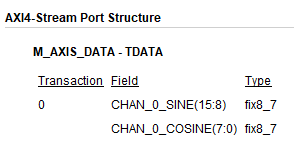
\includegraphics[width=0.45\textwidth]{img/diseno/dds.PNG}
    \caption{Configuración de salida de las señales sinusoidales en el bloque DDS}
    \label{fig:dds}
\end{figure}

\section{Generación de las componentes I/Q y suma}

Para generar las componentes I/Q de transmisión se deben multiplicar las salidas I/Q del filtrado realizado anteriormente por las funciones coseno/-seno generadas en el bloque DDS. Como se ha introducido, el procesamiento de los datos del filtro y el bloque de multiplicación trabajarán a una frecuencia de 576 MHz, siendo el triple de la empleada en los bloques anteriores. 

\vspace{3mm}

Para las salidas I/Q del filtrado (\textit{Salida\_RRC\_I} y \textit{Salida\_RRC\_Q}), es preciso extraer los datos a partir de la lectura de los ficheros \textit{FIR\_output\_I.txt} y \textit{FIR\_output\_Q.txt}, generados anteriormente. A continuación, se muestra el proceso de lectura en el caso de la rama I.

\pagebreak

\begin{lstlisting}[language=VHDL, style=mystyle, caption={Proceso de lectura del fichero de salida del filtrado (rama I)}]
process(clk) 
    --lectura datos salidas filtros
    variable line_buffer : line;
    variable nuevo_valor : integer;
        
    begin
        if rst = '0' then
            eof_I <= false; --se reinicia fin de archivo
        elsif rising_edge(clk) then 
            if not eof_I then
                if endfile(file_handle_I) then 
                    eof_I <= true; 
                elsif m_axis_data_tvalid_0 = '1' then
                    readline(file_handle_I, line_buffer);
                    read(line_buffer, nuevo_valor);
                    Salida_RRC_I <= std_logic_vector(to_signed(nuevo_valor, Salida_RRC_I'length));
                end if;
            end if;
        end if;    
end process;  
\end{lstlisting}

\vspace{3mm}

Como proceso final, se deben combinar las dos componentes I/Q generadas a la salida de los multiplicadores en un bloque sumador. Este se configurará con dos entradas de 32 bits (C y CONCAT) y una salida de 33 bits.


\section{Comprobación de funcionamiento del mezclador}

En el testbench se añade el proceso principal para activar y desactivar la señal de reset, que irá conectada al bloque DDS y de la cual también dependerá el comienzo de lectura de los ficheros de datos del filtro. Es imprescindible configurarlo de esta manera para que se realice tanto la generación de las ondas sinusoidales como la lectura del filtrado de forma simultánea para poder operar.

\vspace{3mm}

\begin{lstlisting}[language=VHDL, style=mystyle, caption={Proceso de estimulación}]
process
begin
    file_open(file_handle_I, ".\FIR_output_I.txt", READ_MODE);
    file_open(file_handle_Q, ".\FIR_output_Q.txt", READ_MODE);
  
  
    rst <= '0'; -- negativo
    wait for 100 ns;
    rst <= '1';               

    wait;
end process;
\end{lstlisting}

%%AQUI FIGURAS FINALES








